\chapter{NNQS exploration}\label{nnqsresults}
This chapter explores the performance of different architectures and training schedules that can be used to train the NNQS solver. All experiments in this section were run on a subset of the entire dataset with problem sizes of $10,25,50,75,200,250$ and $10$ problems for each problem type and size. 

%The problem evaluation metrics are also calculated by considering the solutions from the different types of NNQS to draw a clearer comparison between architectures and training schemes.

\section{Architectures and Training Schedules}
We will utilise the Restricted Boltzmann Machine (RBM) and the Multilayer Perceptron (MLP) as the architecture for NNQS. For a given input problem with $n$ variables, the RBM model will have $n$ visible nodes and $5n$ hidden nodes, while the MLP will have $n$ input nodes, $1$ hidden layer of size $5n$ and $1$ positive real output node. The RBM uses the sigmoid function, while the MLP uses the ReLU activation function and a sigmoid function as the output function. We use Gibbs sampling for the RBM and Metropolis sampling for the MLP which are detailed in \autoref{samplingmethods}.

We will also compare three training schedules for the NNQS solver---progressive, direct, and continuous. The progressive training algorithm follows \autoref{alg:progressiveagain} and has been utilised in previous experiments. In progressive training, the normalised anneal fraction $s$ is incremented by $0.1$, and the NNQS is trained until convergence each time. In direct training, described in \autoref{alg:direct}, $s$ is held constant at $1$ for all epochs. In continuous training, described in \autoref{alg:continuous}, $s$ is gradually increased every iteration and the NNQS is not trained to convergence. All schedules use at most $1000$ iterations.

\begin{algorithm}
    \begin{algorithmic}
    \For {$s \in [0.1, 1.0]$ step $0.1$}
    \State Set $H(s) \leftarrow A(s)\hat{H}_0 + B(s)\hat{H}_c$;
    \State Train NNQS on $H(s)$ until convergence or until epoch limit of $100$ is reached;
    \EndFor
    \end{algorithmic}
    \caption{NNQS Progressive Schedule}
    \label{alg:progressiveagain}
\end{algorithm}

\begin{algorithm}
    \begin{algorithmic}
    \State Set $H \leftarrow B(1)\hat{H}_c$;
    \State Train NNQS on $H$ until convergence or until epoch limit of $1000$ is reached;
    \end{algorithmic}
    \caption{NNQS Direct Schedule}
    \label{alg:direct}
\end{algorithm}

\begin{algorithm}
    \begin{algorithmic}
    \For {$s \in [0.001, 1.0]$ step $0.001$}
    \State Set $H(s) \leftarrow A(s)\hat{H}_0 + B(s)\hat{H}_c$;
    \State Train NNQS on $H(s)$ for $1$ epoch;
    \EndFor
    \end{algorithmic}
    \caption{NNQS Continuous Schedule}
    \label{alg:continuous}
\end{algorithm}

Direct training is a baseline for training a neural network with the cost function as the problem Hamiltonian for the entire training period. Progressive training most closely resembles the quantum annealing process, where the system is kept at the ground state by training until convergence after each increment of $s$. Continuous training slowly increments $s$ but does not train until convergence.

\section{Results and Discussion}
We present the performance metrics for each dataset, accompanied by error bars representing the unbiased standard error of the mean. Graphs with problem sizes on the x-axis are plotted with a log scale. The performance by dataset and problem size is shown in \autoref{appendix:nnqssizegraph}.

\subsection{NAE3SAT}
For the NAE3SAT dataset, the continuous training scheme with the RBM performs the best in average performance and success probability when averaged across all problem sizes, shown in \autoref{nnqs-nae3sat-average}. The RBM, with progressive training, and the MLP, with continuous training, also perform well.

\begin{figure}[!htb]
    \centering
    \subfloat[Normalized energy]{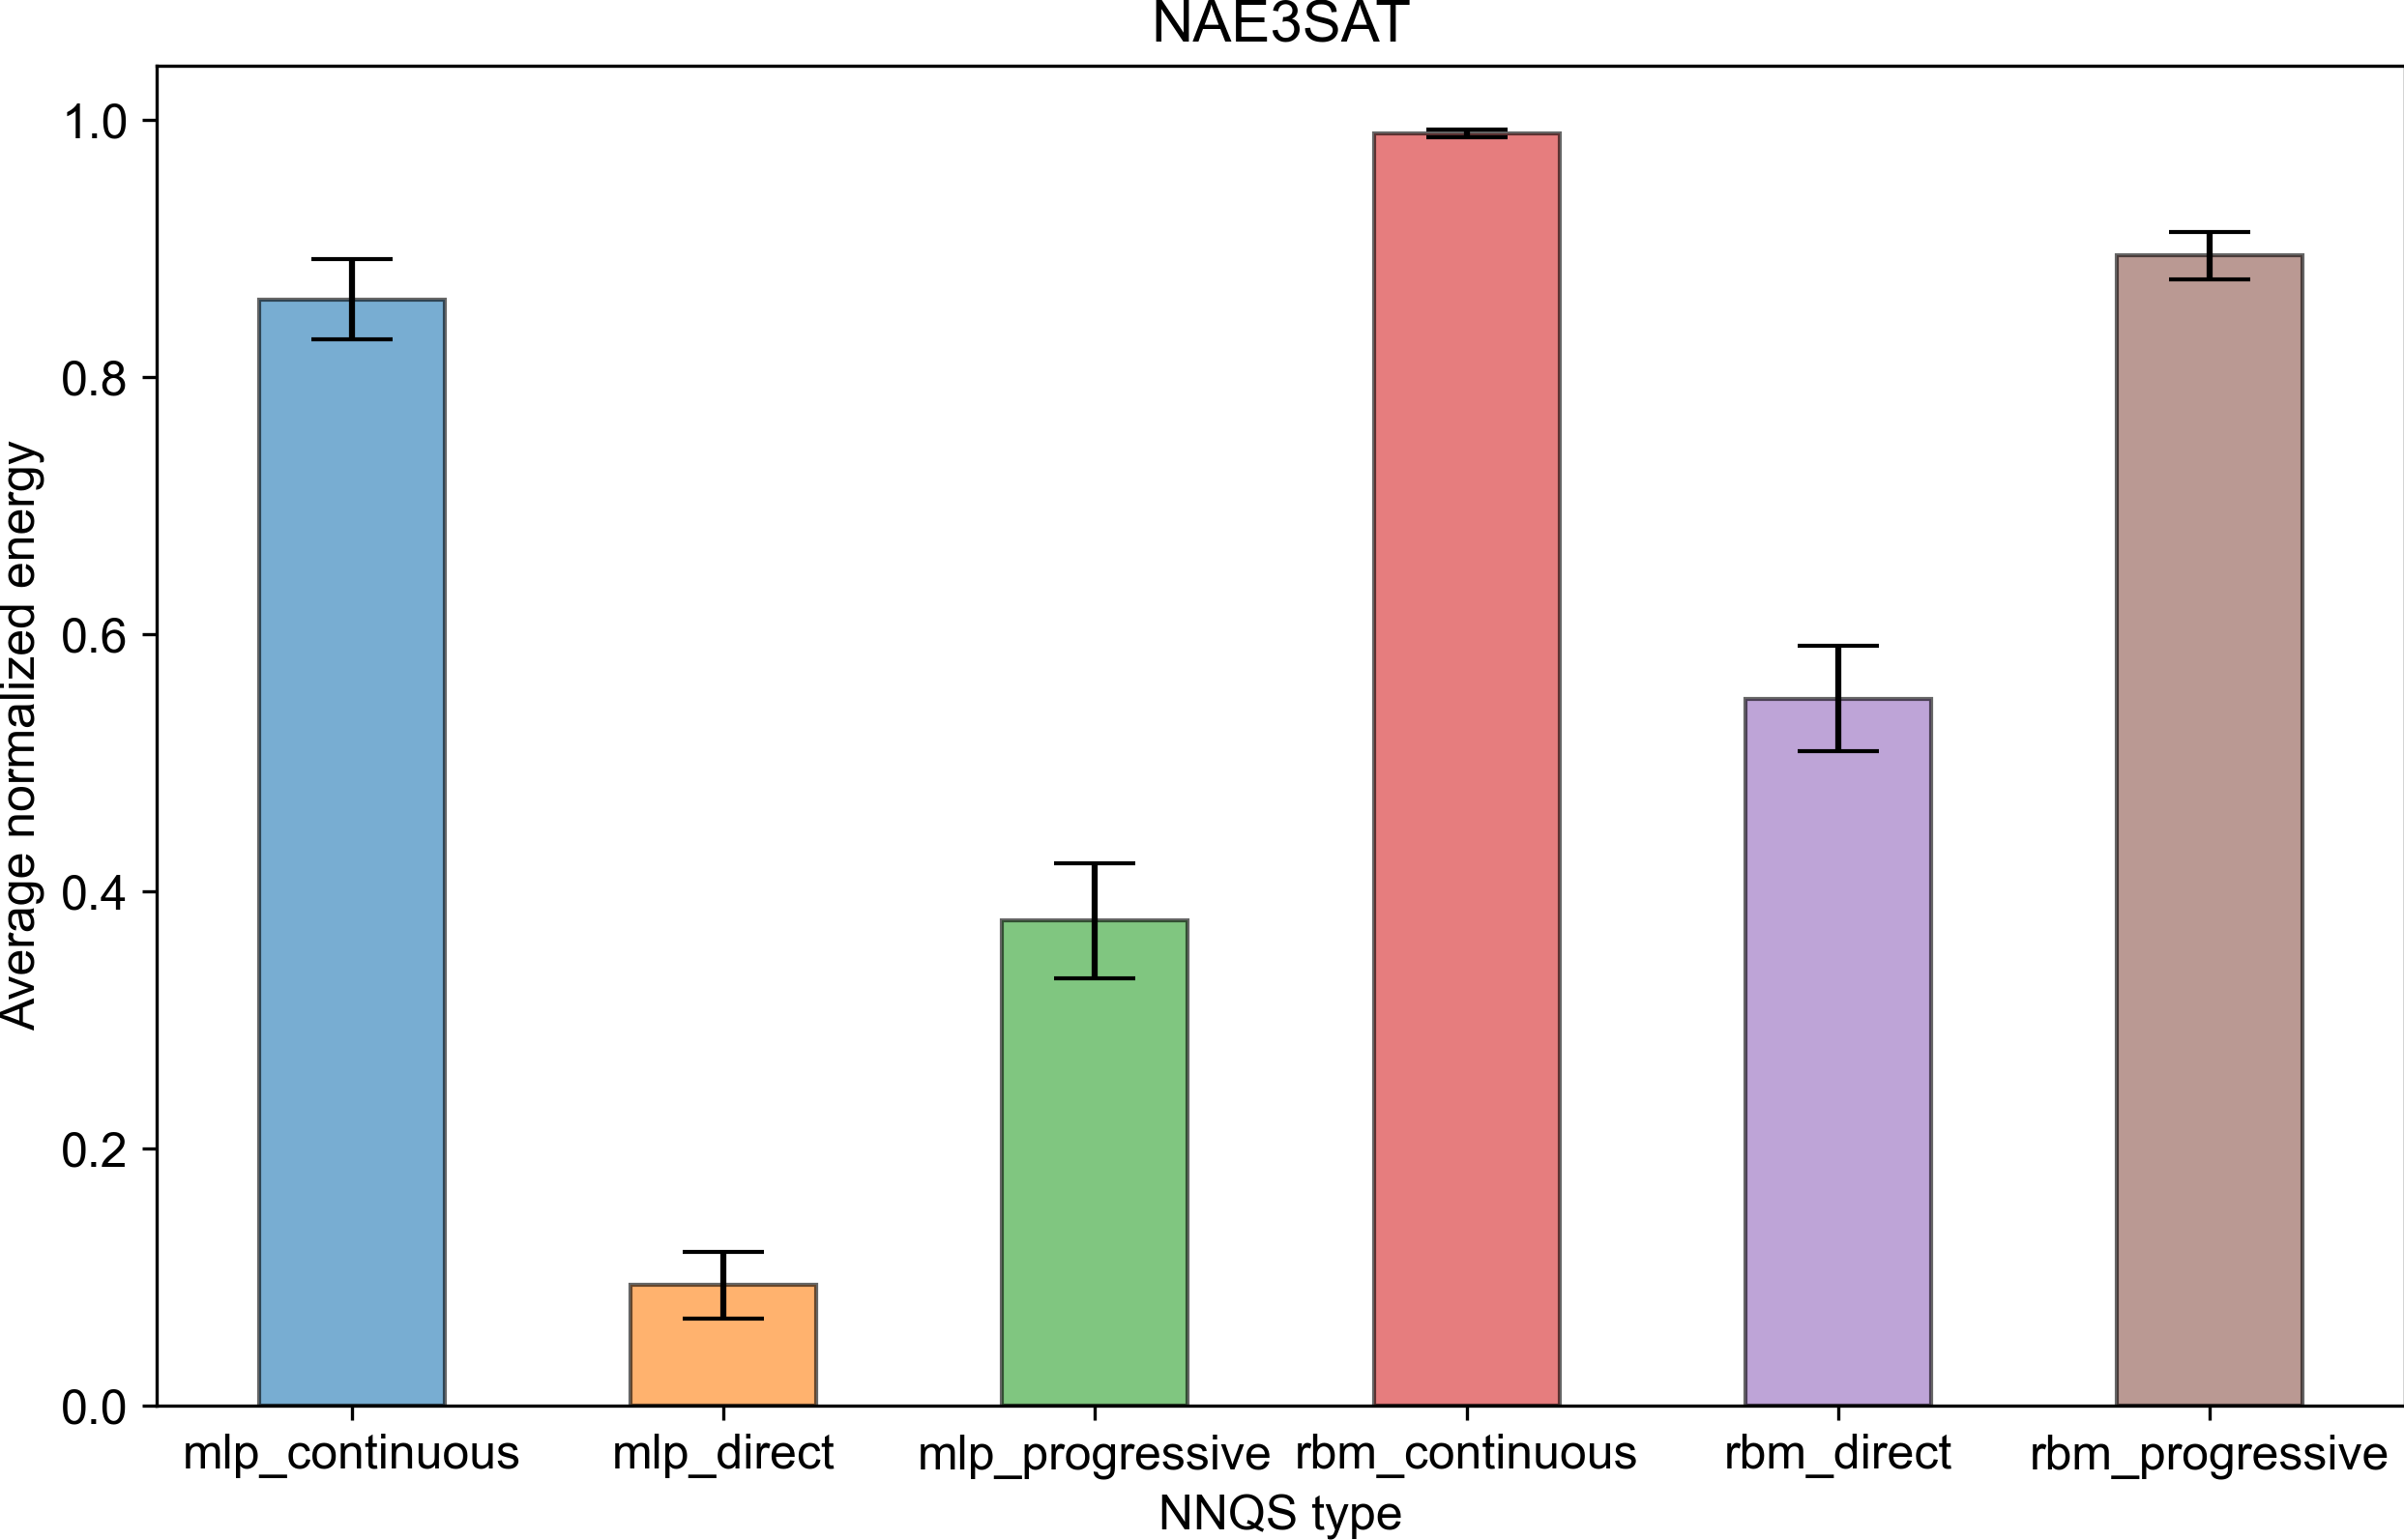
\includegraphics[width=0.5\textwidth]{images/nae3sat_nnqs_avg.png}}
    \subfloat[Success probability]{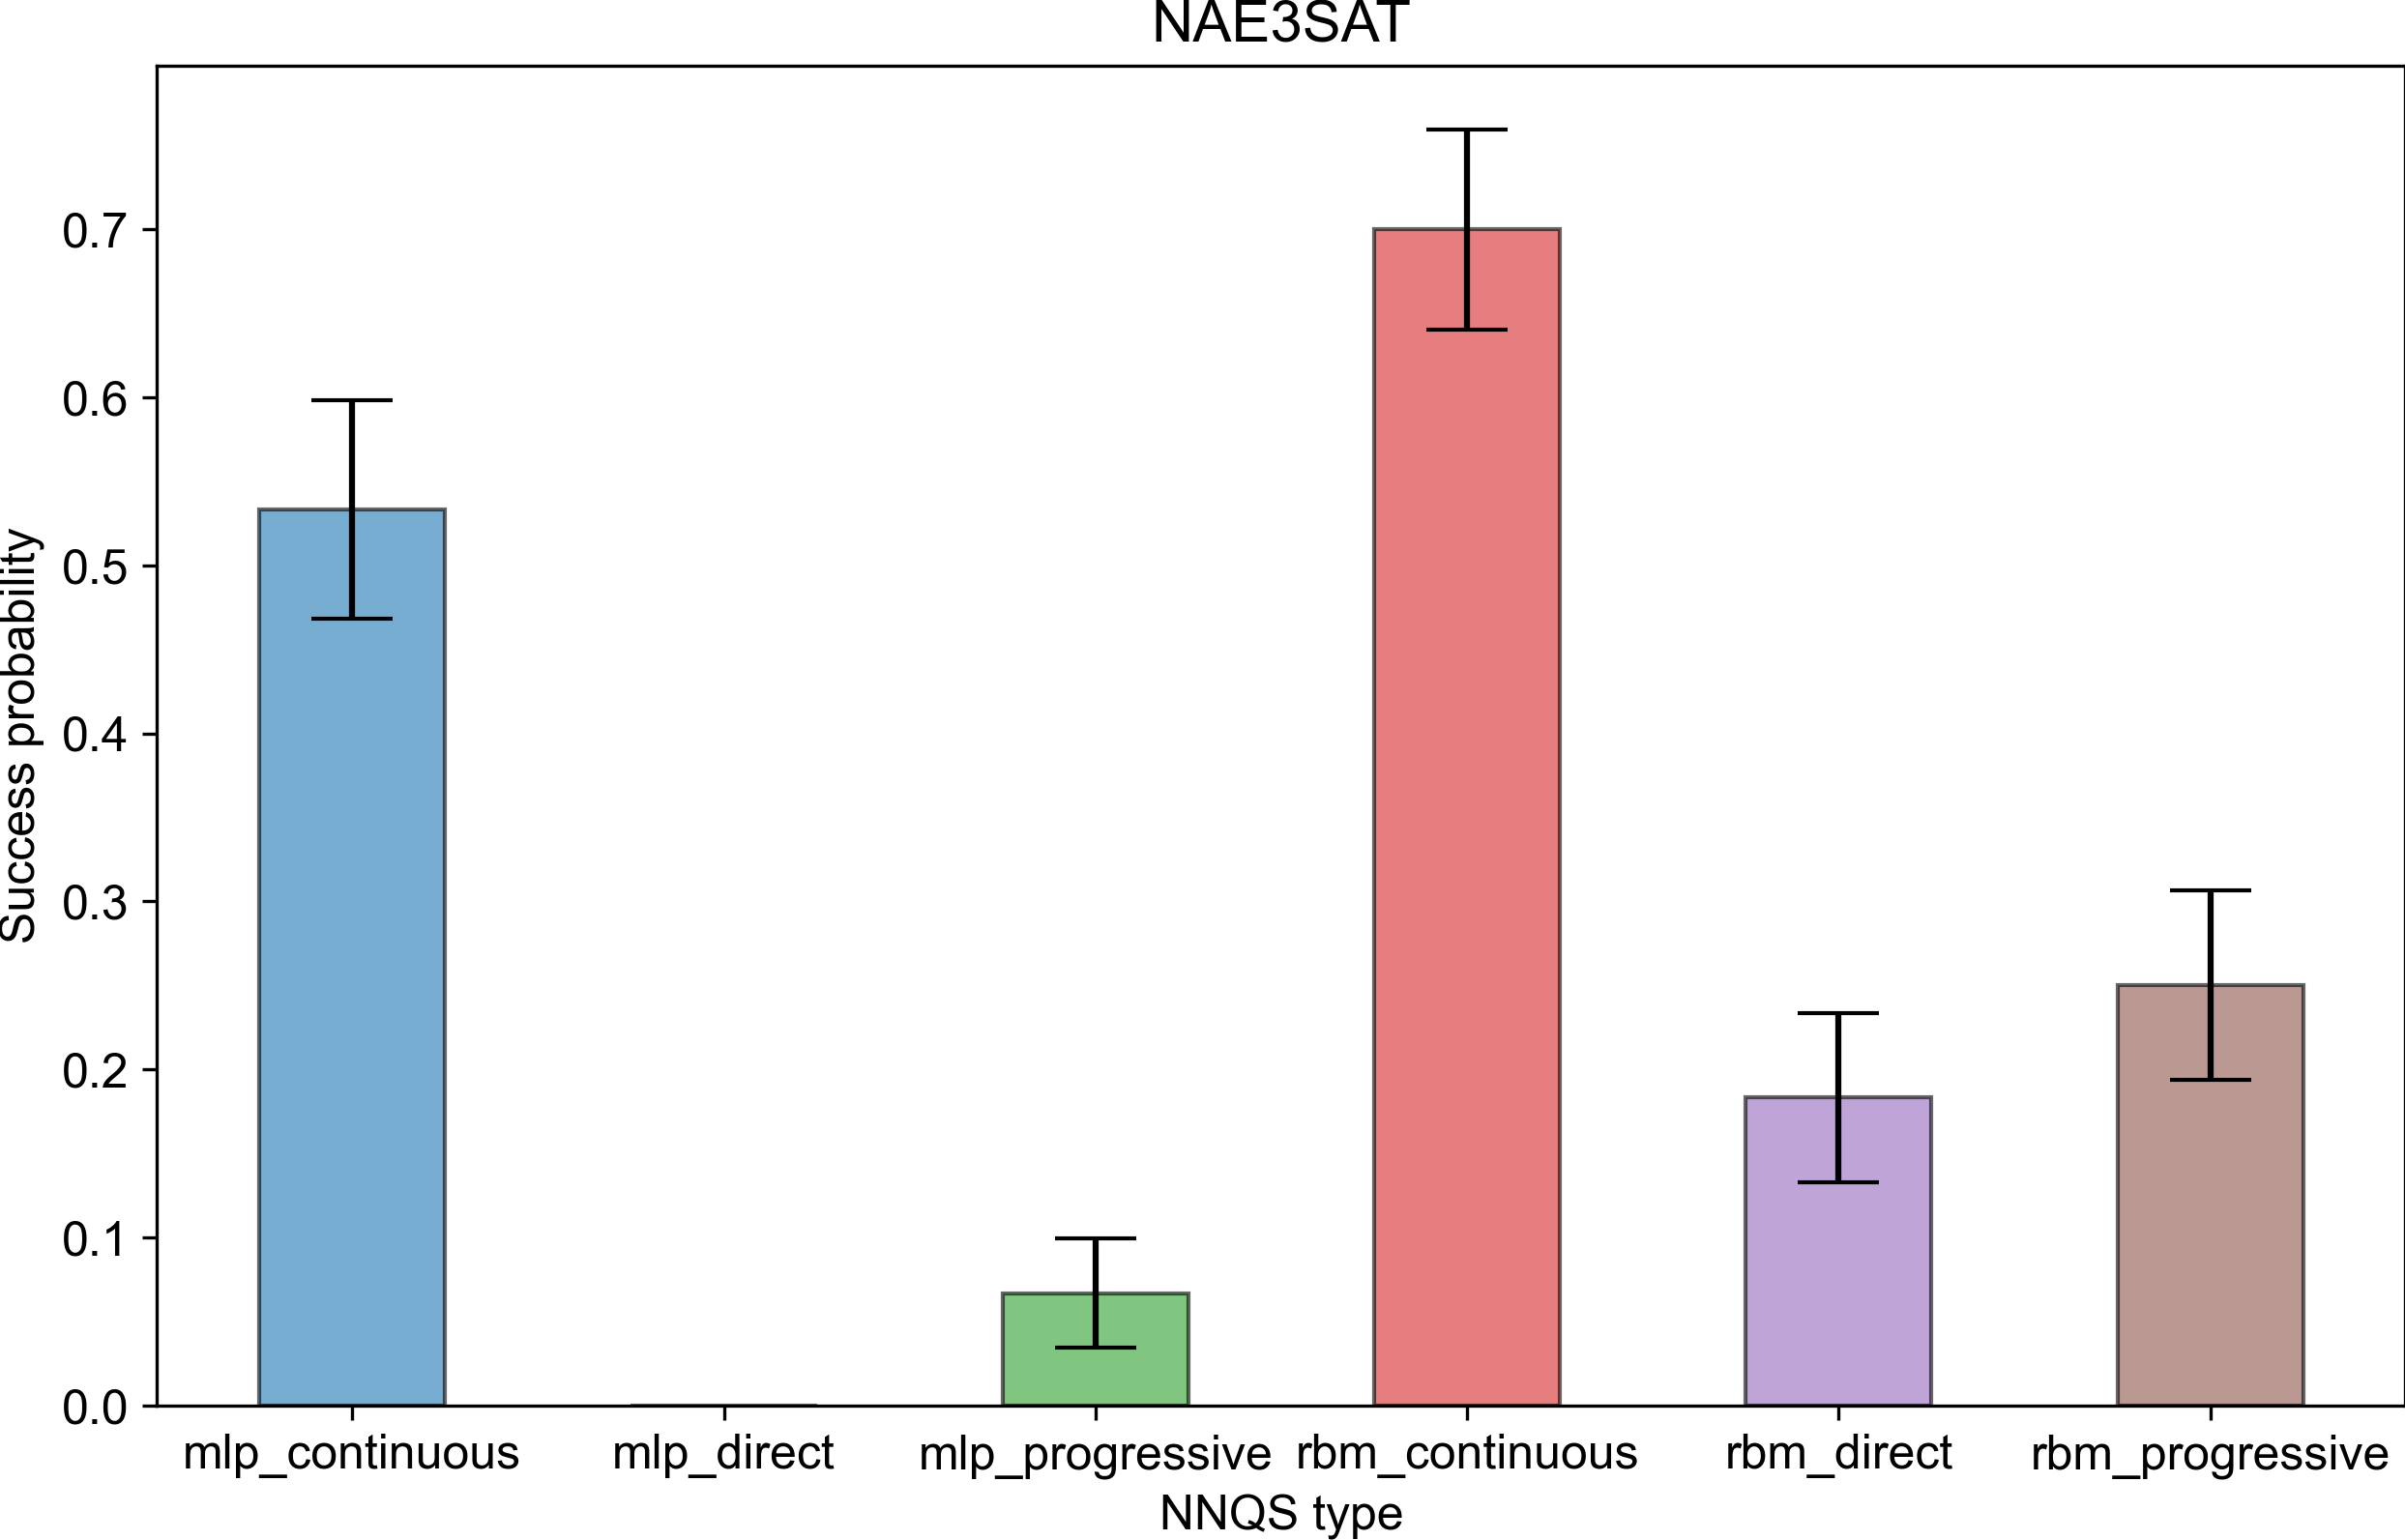
\includegraphics[width=0.5\textwidth]{images/nae3sat_nnqs_success_avg.png}}
    \caption{Average performance of different NNQS types for NAE3SAT}
    \label{nnqs-nae3sat-average}
\end{figure}

\subsection{Max-cut}
For the maxcut dataset, the continuous training algorithm with the RBM again performs the best in average performance and success probability when averaged across all sizes, shown in \autoref{nnqs-maxcut-average}. The RBM, with progressive training, and the MLP, with continuous training, also perform well. However, the performance gap between the top three solvers is relatively small, implying that the max-cut problem is easier than the NAE3SAT problem.

\begin{figure}[!htb]
    \centering
    \subfloat[Normalized energy]{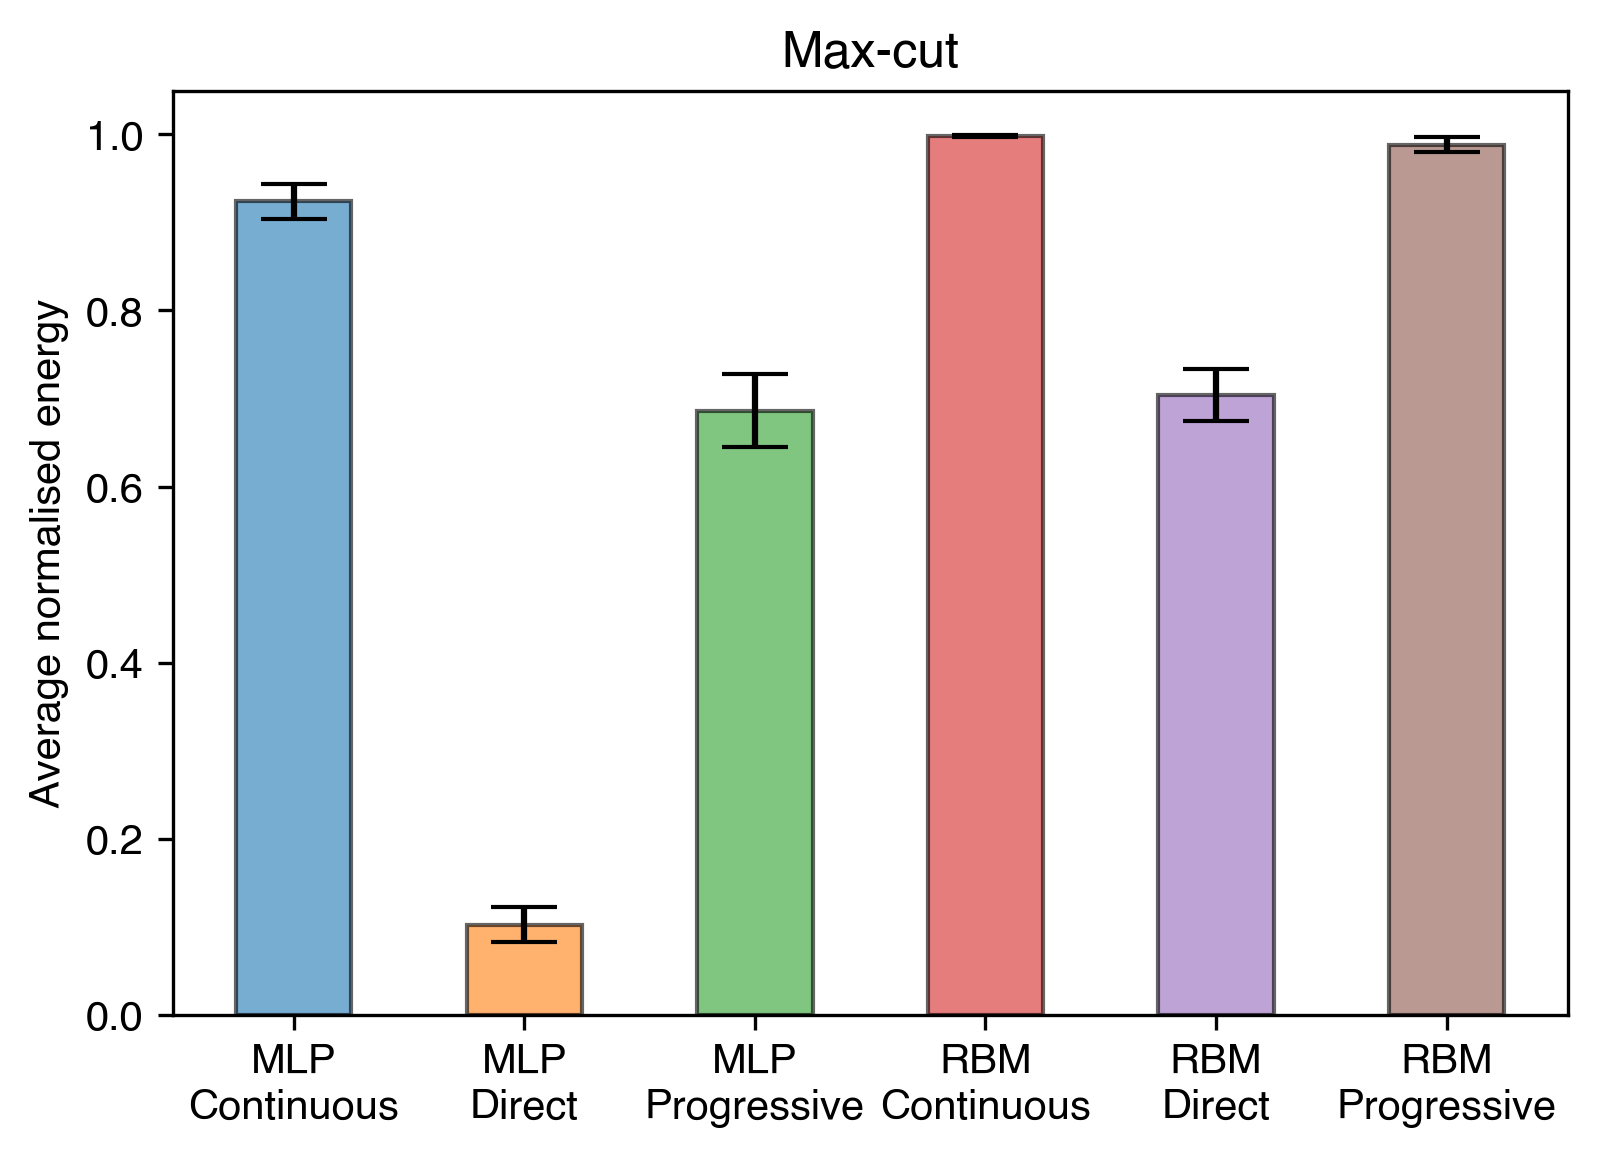
\includegraphics[width=0.5\textwidth]{images/maxcut_nnqs_avg.png}}
    \subfloat[Success probability]{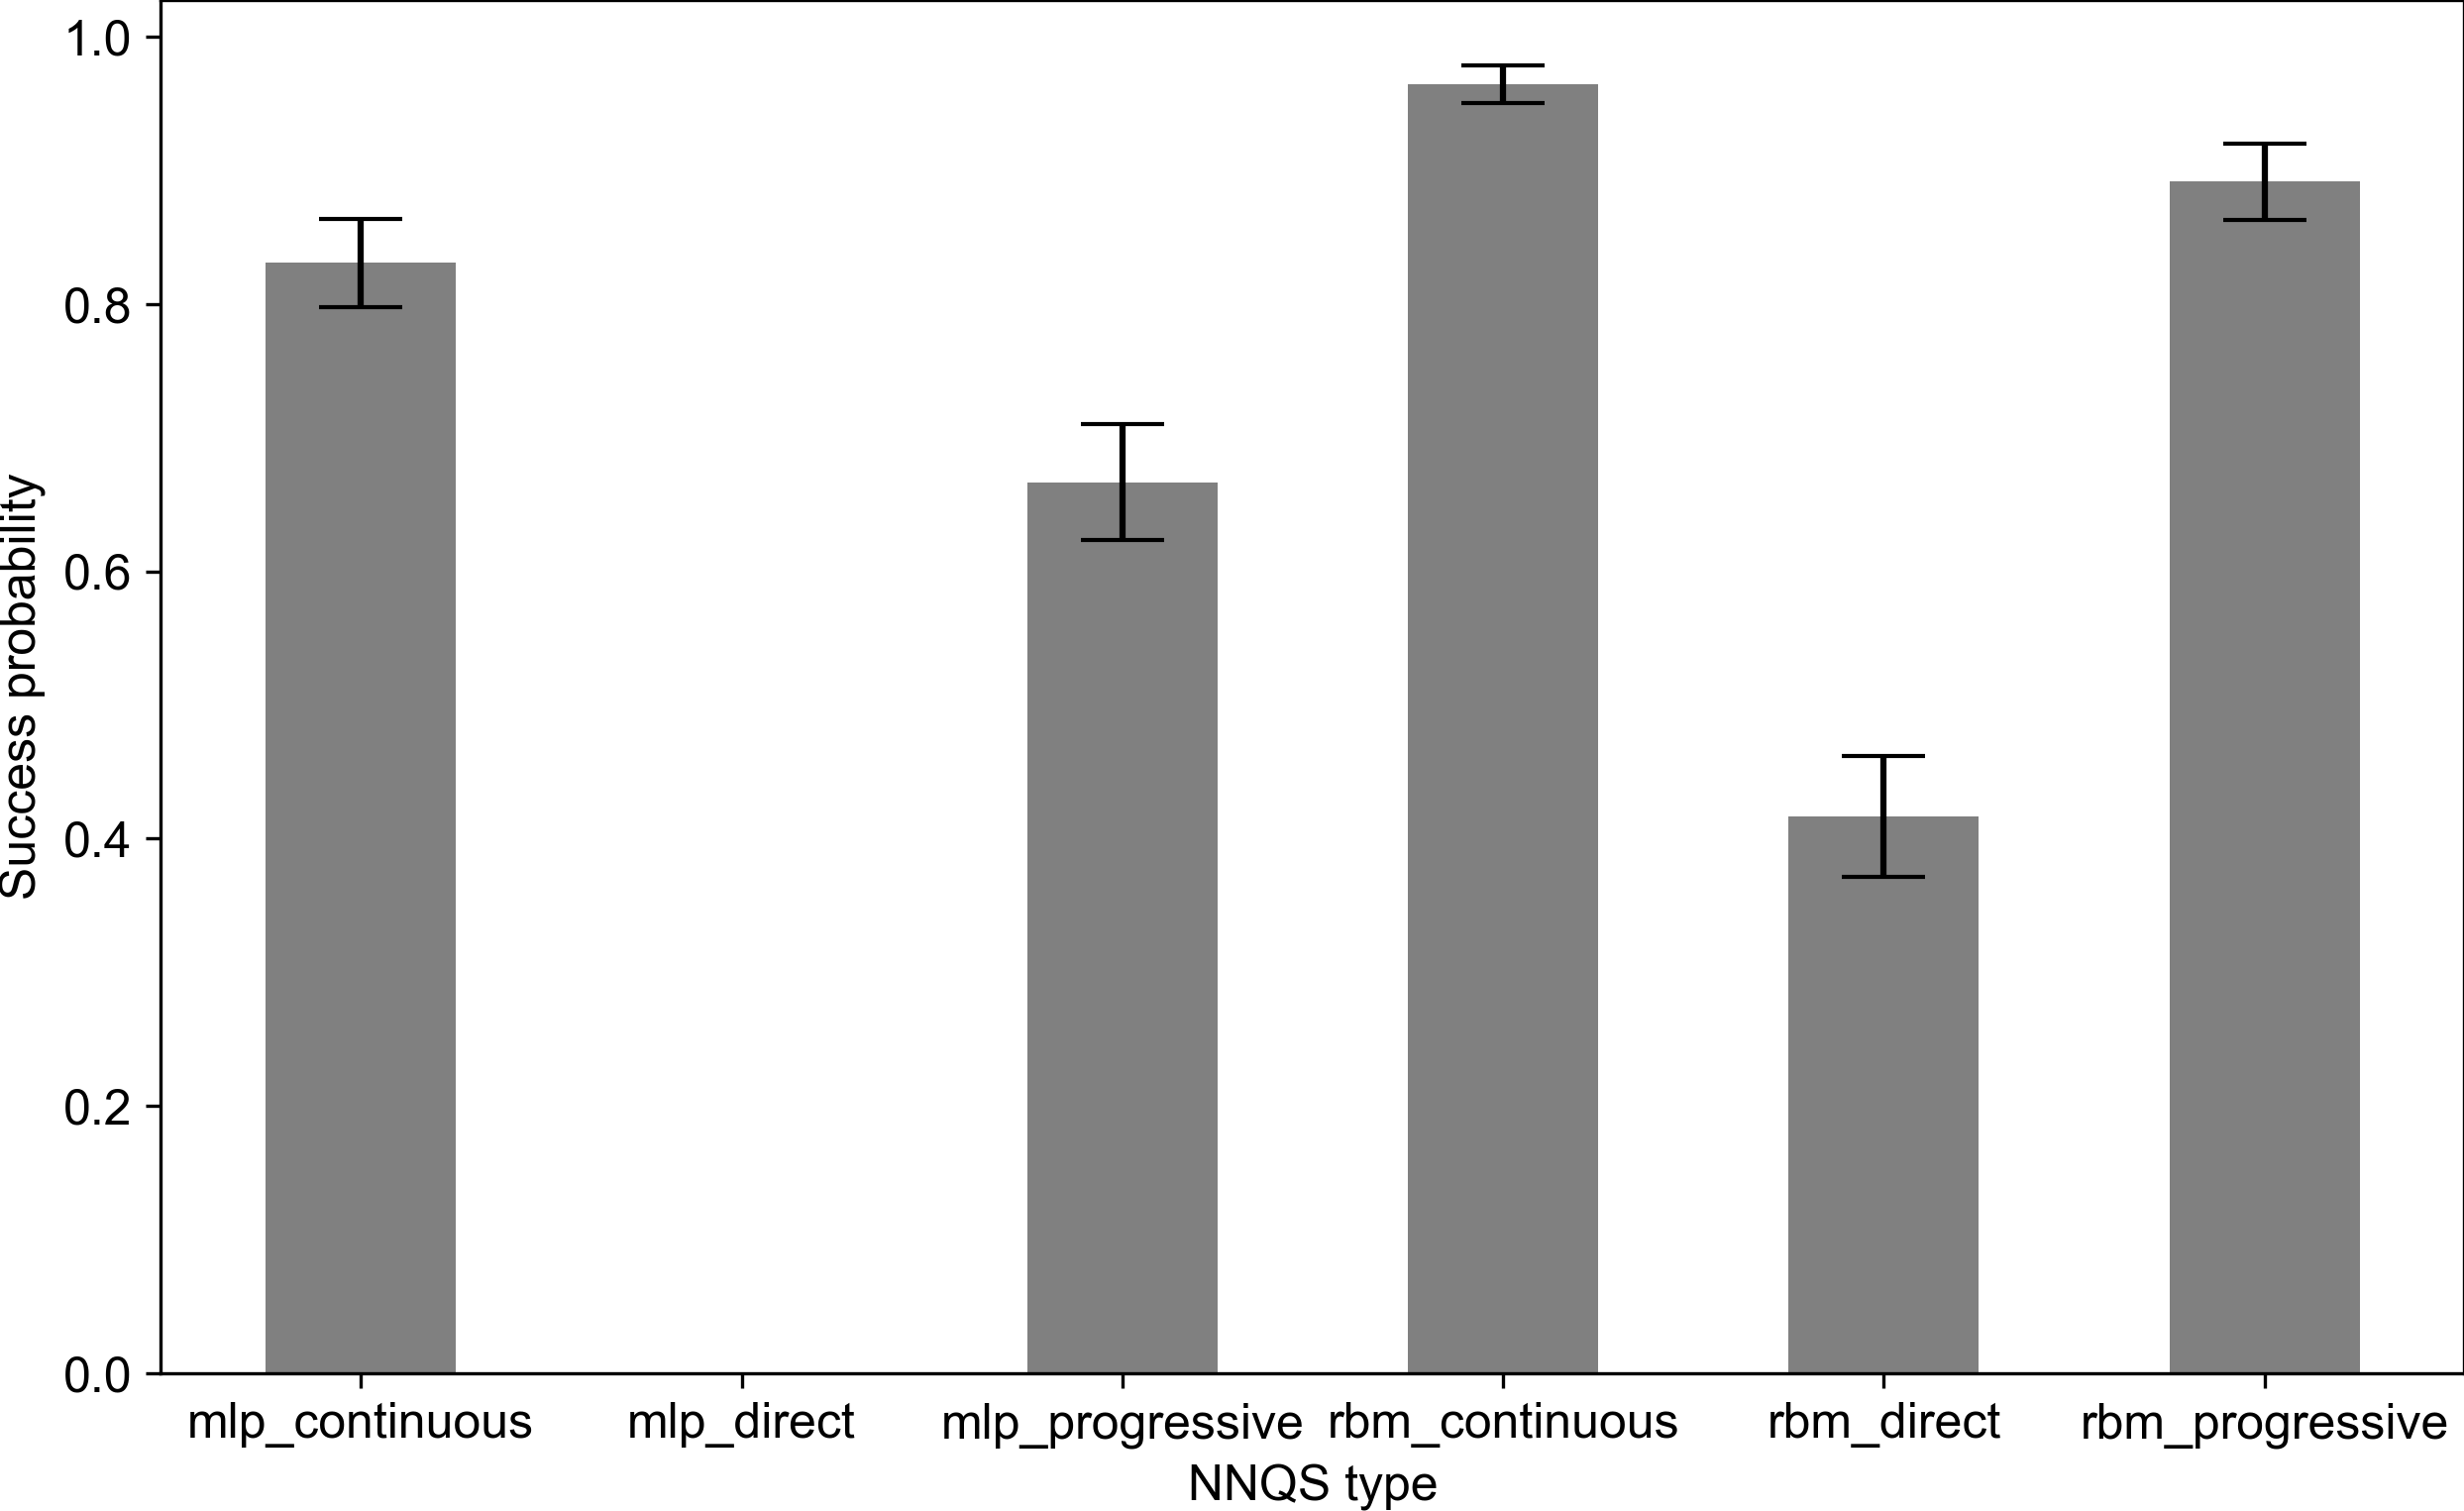
\includegraphics[width=0.5\textwidth]{images/maxcut_nnqs_success_avg.png}}
    \caption{Average performance of different NNQS types for max-cut}
    \label{nnqs-maxcut-average}
\end{figure}

\subsection{SK model}
For the SK model dataset, the continuous training algorithm with the RBM again performs the best in average performance and success probability when averaged across all sizes, shown in \autoref{nnqs-skmodel-average}. The RBM, with progressive training also perform well in both metrics.

\begin{figure}[!htb]
    \centering
    \subfloat[Normalized energy]{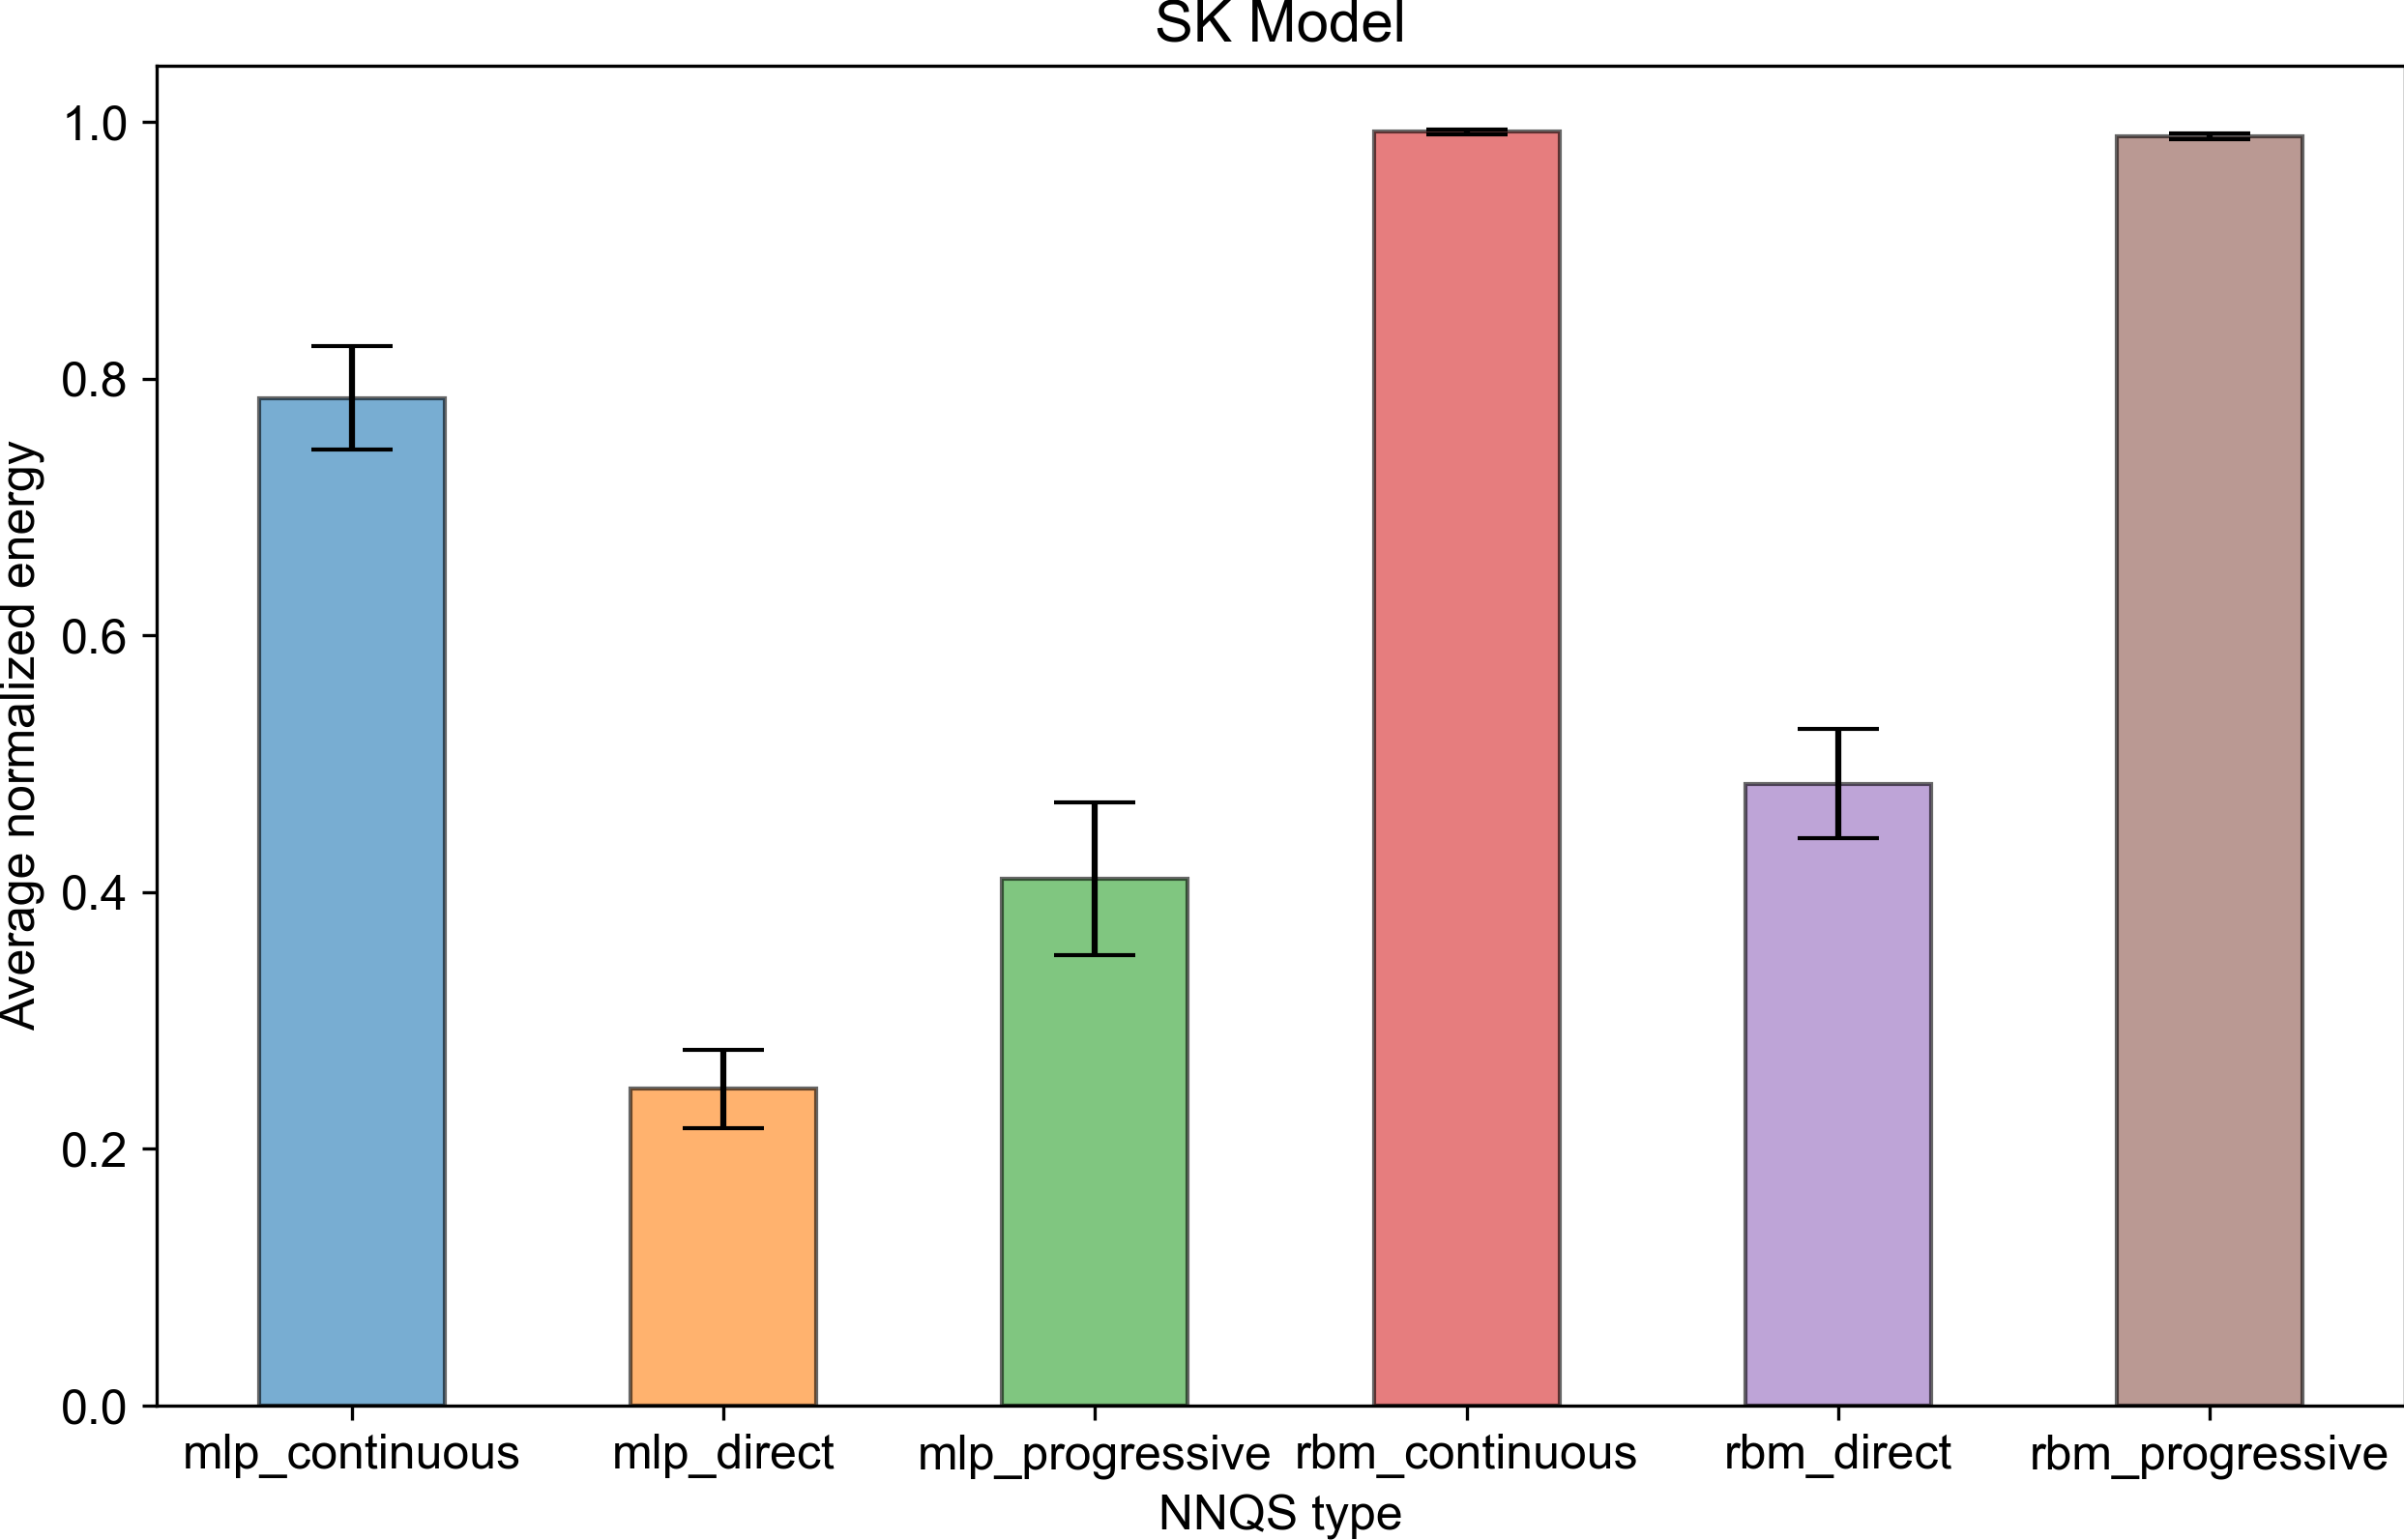
\includegraphics[width=0.5\textwidth]{images/skmodel_nnqs_avg.png}}
    \subfloat[Success probability]{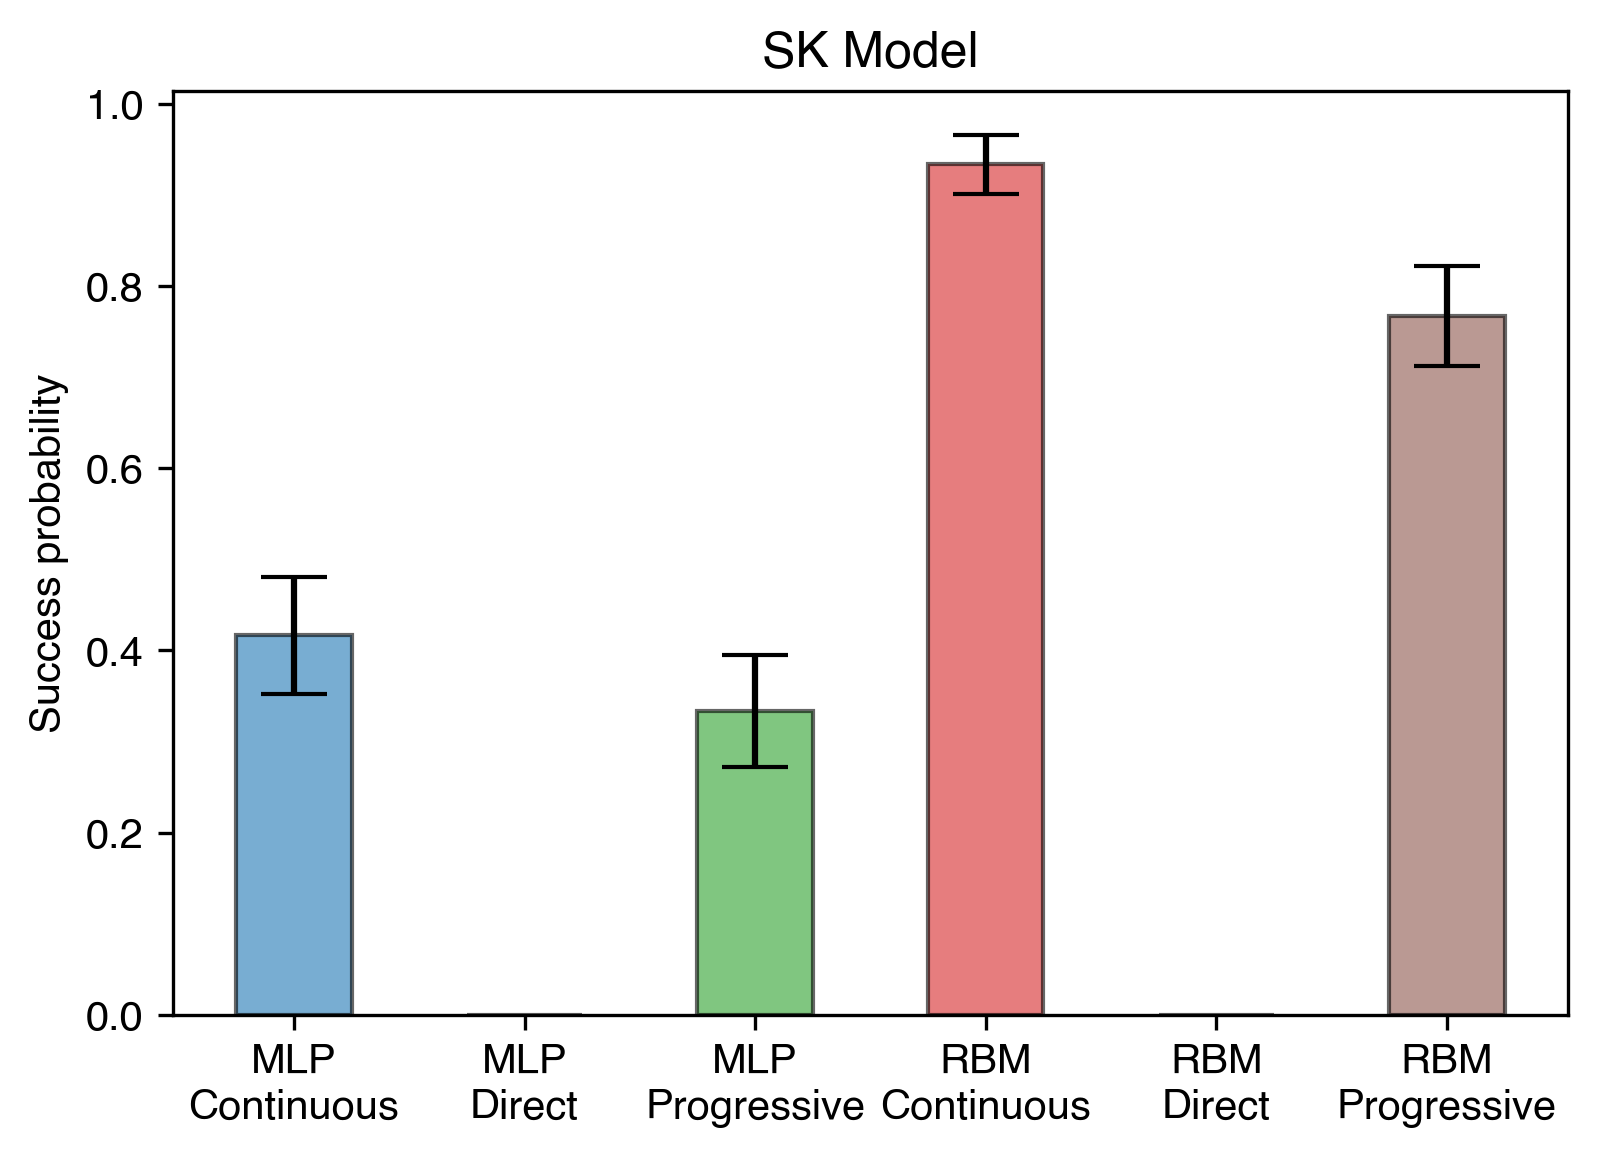
\includegraphics[width=0.5\textwidth]{images/skmodel_nnqs_success_avg.png}}
    \caption{Average performance of different NNQS types for SK model}
    \label{nnqs-skmodel-average}
\end{figure}

\section{Conclusion}
\autoref{results:nnqsnormalizedenergy} and \autoref{results:nnqssuccess} summarises the average normalised energy and success probability for different types of NNQS for each dataset and also the average across all datasets.

Comparing the two architectures, RBM performs better than MLP in average normalised energy and success probability for all datasets and training schemes. In terms of training schemes, direct training performs the worst among the three, and continuous training performs slightly better than progressive training. Using the RBM with a continuous training scheme gives the highest normalised energy and success probability across all datasets. 

The RBM likely performs better as it uses Gibbs sampling, which helps the neural network approximate the wave function more closely. The Gibbs sampling method also allows for multiple-bit flips in each iteration and is thus able to explore a larger state space.

Even though progressive training more closely mimics the quantum annealing process in D-wave solvers, the sudden change of Hamiltonian may have led to large gradient terms that may have made it more difficult for the network to converge, leading to poorer training. Continuous training gradually changes the Hamiltonian, which limits the gradient magnitudes and may result in better training. Direct training is expected to perform poorly as it tends to get stuck in local minima.


\begin{table}[!htb]
    \centering
    \begin{tabular}{ccccccc} \toprule
        ~ & \multicolumn{3}{c}{MLP} & \multicolumn{3}{c}{RBM} \\
        \cmidrule{2-7} & Continuous & Direct & Progressive & Continuous & Direct & Progressive \\
        \midrule
        NAE3SAT & 0.866 & 0.118 & 0.352 & \textbf{0.997} & 0.511 & 0.910 \\
        Max-cut & 0.924 & 0.102 & 0.686 & \textbf{0.998} & 0.704 & 0.988 \\
        SK model & 0.790 & 0.248 & 0.411 & \textbf{0.999} & 0.488 & 0.995 \\ \midrule
        Average & 0.860 & 0.156 & 0.483 & \textbf{0.998} & 0.568 & 0.965 \\ \bottomrule
    \end{tabular}
    \caption{Average normalised energy for different NNQS types}
    \label{results:nnqsnormalizedenergy}
\end{table}

\begin{table}[!htb]
    \centering
    \begin{tabular}{ccccccc} \toprule
        ~ & \multicolumn{3}{c}{MLP} & \multicolumn{3}{c}{RBM} \\
        \cmidrule{2-7} & Continuous & Direct & Progressive & Continuous & Direct & Progressive \\
        \midrule
        NAE3SAT & 0.583 & 0.029 & 0.062 & \textbf{0.950} & 0.167 & 0.364 \\
        Max-cut & 0.831 & 0.000 & 0.667 & \textbf{0.965} & 0.417 & 0.892 \\
        SK model & 0.417 & 0.000 & 0.333 & \textbf{0.933} & 0.000 & 0.767 \\ \midrule
        Average & 0.610 & 0.010 & 0.354 & \textbf{0.949} & 0.194 & 0.674 \\ \bottomrule
    \end{tabular}
    \caption{Success probability for different NNQS types}
    \label{results:nnqssuccess}
\end{table}